\documentclass[tikz,border=5pt]{standalone}
\usepackage{tikz}
\definecolor{blueC}{RGB}{30,90,220}
\definecolor{purpC}{RGB}{125,40,170}
\definecolor{greenC}{RGB}{0,140,60}
\definecolor{orangeC}{RGB}{255,140,40}

\usetikzlibrary {arrows.meta}

\begin{document}
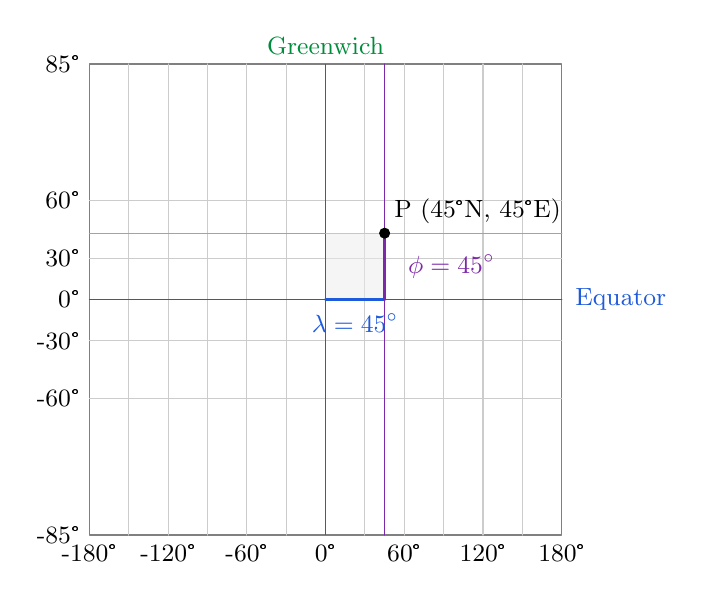
\begin{tikzpicture}[line cap=round, line join=round]

% ================= Panel 2: Pseudo-Mercator map =================
% x = lambda/60 cm, y = 0.955 * ln(tan(45 + phi/2)), map spans lat -85 to +85
\draw[gray, thin] (0,-2.991) rectangle (6,2.991);

% Grid: meridians every 30 deg, parallels every 30 deg
\foreach \l in {-150,-120,-90,-60,-30,0,30,60,90,120,150}
  \draw[gray!40, thin] (3+\l/60,-2.991) -- (3+\l/60,2.991);
\foreach \y in {1.258,0.524,-0.524,-1.258}
  \draw[gray!40, thin] (0,\y) -- (6,\y);

% Latitude labels
\node[left, font=\small] at (0,2.991) {85°};
\node[left, font=\small] at (0,1.258) {60°};
\node[left, font=\small] at (0,0.524) {30°};
\node[left, font=\small] at (0,0) {0°};
\node[left, font=\small] at (0,-0.524) {-30°};
\node[left, font=\small] at (0,-1.258) {-60°};
\node[left, font=\small] at (0,-2.991) {-85°};

% Longitude labels along the bottom edge
\node[below, font=\small] at (0,-2.991) {-180°};
\node[below, font=\small] at (1,-2.991) {-120°};
\node[below, font=\small] at (2,-2.991) {-60°};
\node[below, font=\small] at (3,-2.991) {0°};
\node[below, font=\small] at (4,-2.991) {60°};
\node[below, font=\small] at (5,-2.991) {120°};
\node[below, font=\small] at (6,-2.991) {180°};
%\node[below, font=\small] at (3.5,-2.991) {30°E};
%\node[below, font=\small] at (2.5,-2.991) {30°W};

% Map cut note
%\node[above left, font=\footnotesize] at (6,2.991) {cut at ±85°};

% Reference lines (thin): equator, Greenwich, 45 E meridian, 45 N parallel
\draw[blueC, thin] (0,0) -- (6,0);
\draw[greenC, thin] (3,-2.991) -- (3,2.991);
\node[greenC, above, font=\small] at (3,2.991) {Greenwich};
\draw[purpC, thin] (3.75,-2.991) -- (3.75,2.991);
\draw[orangeC, thin] (0,0.842) -- (6,0.842);
\node[blueC, anchor=west, font=\small] at (6.05,0) {Equator};

% Rectangle: projection of the 0-45 E, 0-45 N patch
\fill[gray!15, opacity=0.5] (3,0) rectangle (3.75,0.842);
%\draw[purpC, thin] (3.5,0.524) rectangle (4,1.258);

% Measured portions (thick): lambda arc, phi arc
\draw[blueC, very thick] (3,0) -- (3.75,0);
\draw[purpC, very thick] (3.75,0) -- (3.75,0.842);

% Point P (45 N, 45 E)
\fill (3.75,0.842) circle (2pt) node[above right, font=\small] {P (45°N, 45°E)};

% Angle labels matching the 3D panel
\node[blueC, font=\small] at (3.375,-0.3) {$\lambda=45^\circ$};
\node[purpC, font=\small] at (4.6,0.42) {$\phi=45^\circ$};

\end{tikzpicture}
\end{document}
